%!TEX TS-program = xelatex
\documentclass[]{friggeri-cv}
\usepackage{afterpage}
\usepackage{hyperref}
\usepackage{color}
\usepackage{xcolor}
\hypersetup{
    pdftitle={Tiago Oliveira de Farias},
    pdfauthor={Tiago Oliveira de Farias},
    pdfsubject={Currículo},
    pdfkeywords={},
    colorlinks=true,       % no lik border color
   allbordercolors=white    % white border color for all
}
\addbibresource{bibliography.bib}
\RequirePackage{xcolor}
\definecolor{pblue}{HTML}{0395DE}

\begin{document}
\header{Tiago O.}{ de Farias}
      {Analista Desenvolvedor de Sistemas PHP}
      
% Fake text to add separator      
\fcolorbox{white}{gray}{\parbox{\dimexpr\textwidth-2\fboxsep-2\fboxrule}{%
.....
}}

% In the aside, each new line forces a line break
\begin{aside}
  \section{Endereço}  	
    Rua Doutor José Bento Corrêa, 545
    Bairro Protásio Alves,
    CEP: 91450-030
    Rio Grande do Sul, Porto Alegre
    ~
  \section{Telefones}
    51 99292 2705
    51 3018 1864
    ~
  \section{E-mail}
    \href{mailto:tiago.farias.poa@gmail.com}{\textbf{tiago.farias.poa@}\\gmail.com}
    ~
  \section{Web \& Git}
    \href{https://github.com/tofarias}{github.com/tofarias}
    \href{https://bitbucket.org/tiagofarias}{bitbucket.org/tiagofarias}
    \href{https://tiagoodefarias.wordpress.com/}{tiagoodefarias.wordpress}
    \href{https://www.facebook.com/groups/laravelrgs}{facebook.com/laravelrgs}
    \href{https://www.linkedin.com/in/tiago-farias1985}{linkedin.com/in/tiago-farias1985}
    ~
  \section{Tecnologias}
    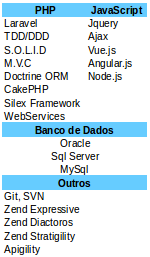
\includegraphics[scale=0.62]{img/programacao.png}
    ~
  \section{Sistemas Operacionais}
    \textbf{GNU/Linux}
\includegraphics[scale=0.40]{img/4stars.png}
    \textbf{Windows}
\includegraphics[scale=0.40]{img/3stars.png}
    ~
  \section{Idiomas}
    \textbf{Espanhol}
\includegraphics[scale=0.40]{img/3stars.png}
    \textbf{Inglês}
\includegraphics[scale=0.40]{img/3stars.png}
\end{aside}

\section{Objetivo}
Atuar no desenvolvimento/análise de sistemas PHP, banco de dados, levantamento de requisítos e métodos ágeis.

\section{Sobre Mim}
Profissional com mais de 6 anos de experiência em desenvolvimento de software. Há alguns anos se empenha no estudo e aplicação de princípios S.O.L.I.D./GRASP e refatoração de código, mais recentemente tem se dedicado ao estudo de \textit{Domain-Driven design} o qual também foi tema do trabalho de conclusão da pós-gradução.
\section{Formação}
\begin{entrylist}
  \entry
    {2014 - 2016}
    {Pós-Graduação: Sist. de Informação com Métodos Ágeis}
    {UniRitter}
    {Tópicos principais: Práticas de Desenvolvimento Ágil, Design Patterns, Smells e Refatoring, Arquiteturas para Web, Testes Ágeis de Software, Gerência de Projetos, Agile Coaching e Mentoring.\\
    \emph{Título do Artigo: "Aplicação de Domain-Driven Design no Gerenciamento de GRU de Cronotacógrafo no Inmetro/RS".} https://github.com/tofarias/artigo-ddd/blob/master/artigo/artigo-domain-driven-design.pdf \\
    \emph{Orientador: M.e. Guilherme Silva de Lacerda.}\\
    Endereço: Rua Orfanotrófio, 555 - Alto Petrópolis, Porto Alegre/RS\\}
  \entry
    {2010 - 2013}
    {Graduação: Análise e Desenvolvimento de Sistemas}
    {Faculdades QI}
    {Tópicos principais: Serviços para Web, Gestão de Projetos, Segurança de Software, Engenharia de Software, Desenvolvimento Java O.O.\\
    Endereço: Av. Julho de Castilhos, 435 - Centro, Porto Alegre/RS\\}    
  \entry
    {2008 - 2010}
    {Técnico: Informática.}
    {Faculdades QI}
    {Endereço: Av. Assis Brasil, 3312 - Porto Alegre/RS}
\end{entrylist}
\section{Certificados/Eventos}
\begin{entrylist}
  \entry
    {Abril/2017}
    {iMasters Certified Professional}
    {iMasters}
    {PHP - Boas práticas\\ \href{http://certificacao.imasters.com.br/users/tiago-oliveira-de-farias}{http://certificacao.imasters.com.br/users/tiago-oliveira-de-farias}}
    \entry
    {2015}
    {TDC - The Developer's Conference}
    {Uniritter}
    {Trilha PHP}
  \entry
    {2012}
    {Semana Acadêmica}
    {Faculdades QI}
    {Participou como painelista - PHP: Codeigniter e Lumine}
  \entry
    {2011}
    {Projeto Crescer}
    {CWI}
    {Treinamento com SQL Server, .Net e Java}
   \entry
    {2011}
    {Treinamento PHP}
    {Target Trust}
    {Treinamento PHP - Zend Framework}
   \entry
    {2011}
    {Trabalho voluntário}
    {Faculdades QI}
    {Trabalho voluntário de monitoria na disciplina de Algoritmos e Programação}
\end{entrylist}
\newpage
\section{Experiência}
\begin{entrylist}
  \entry
    {03/2015 - hoje}
    {Analista/Programador PHP}
    {Advanced IT}
    {Alocado no cliente Inmetro. Atua principalmente com a linguagem PHP (CakePHP) e banco de dados Oracle no projeto Cronotacógrafo. Realiza desde o levantamento de requisitos através de entrevistas com usuário até a análise de impacto juntamente com os administradores de banco de dados.\\}
 \entry
    {08/2013 - 03/2015}
    {Analista de Sistemas}
    {Construtora Pelotense}
    {Atuou no desenvolvimento de sistema web interno que tem por objetivo gerenciar contratos e faturas das obras. O módulo de faturas é carregado com informações da base de dados (SQL Server) gerenciada pelo sistema da TOTVS: RM e Fluxos. Desenvolveu com PHP (Laravel), TDD, Git, em ambiente linux juntamente com banco de dados MySql.\\}
    \entry
    {01/2013 - 08/2013}
    {Programador}
    {Constat}
    {Atuou principalemten com a linguagem PHP. Responsável por desenvolver soluções para o produto Qualitor e seus módulos. Realizava análise de requisitos, documentação de projeto, desenvolvimento com TDD.}
    \entry
    {05/2012 - 12/2012}
    {Técnico em Informática}
    {EMATER-RS/ASCAR}
    {Ingressou mediante concurso público, atuando na manutenção de computadores nos escritórios municipais. Eventualmente desenvolveu programas em Java para auxiliar nas demandas do setor.}
    \entry
    {05/2011 - 04/2012}
    {Programador}
    {CWI}
    {Ingressou em abril/2011 no projeto “Crescer” da empresa CWI Software que ocorreu em São Leopoldo, o
treinamento com duração de 2 meses envolveu as seguintes tecnologias: SQL Server 2008, ASP.Net, C Sharp, Java Web.\\
Com o término do projeto “Crescer” continuou na empresa como estagiário trabalhando no suporte técnico na sede São Leopoldo com PHP/Zend Framework para o cliente “TUV Rheinland” e CodeIgniter para o cliente Terra, foi transferido para a unidade em Porto Alegre ingressando no projeto do cliente “Odebrecht”, utilizando as tecnologias dotNet MVC e PL/SQL, após ingressou na equipe de desenvolvimento para o cliente SENAC/RS no projeto para desenvolver a intranet da empresa utilizando dotNET MVC e SqlServer 2008.}
\end{entrylist}
\end{document}